\documentclass[twoside]{book}

% Packages required by doxygen
\usepackage{fixltx2e}
\usepackage{calc}
\usepackage{doxygen}
\usepackage[export]{adjustbox} % also loads graphicx
\usepackage{graphicx}
\usepackage[utf8]{inputenc}
\usepackage{makeidx}
\usepackage{multicol}
\usepackage{multirow}
\PassOptionsToPackage{warn}{textcomp}
\usepackage{textcomp}
\usepackage[nointegrals]{wasysym}
\usepackage[table]{xcolor}

% Font selection
\usepackage[T1]{fontenc}
\usepackage[scaled=.90]{helvet}
\usepackage{courier}
\usepackage{amssymb}
\usepackage{sectsty}
\renewcommand{\familydefault}{\sfdefault}
\allsectionsfont{%
  \fontseries{bc}\selectfont%
  \color{darkgray}%
}
\renewcommand{\DoxyLabelFont}{%
  \fontseries{bc}\selectfont%
  \color{darkgray}%
}
\newcommand{\+}{\discretionary{\mbox{\scriptsize$\hookleftarrow$}}{}{}}

% Page & text layout
\usepackage{geometry}
\geometry{%
  a4paper,%
  top=2.5cm,%
  bottom=2.5cm,%
  left=2.5cm,%
  right=2.5cm%
}
\tolerance=750
\hfuzz=15pt
\hbadness=750
\setlength{\emergencystretch}{15pt}
\setlength{\parindent}{0cm}
\setlength{\parskip}{3ex plus 2ex minus 2ex}
\makeatletter
\renewcommand{\paragraph}{%
  \@startsection{paragraph}{4}{0ex}{-1.0ex}{1.0ex}{%
    \normalfont\normalsize\bfseries\SS@parafont%
  }%
}
\renewcommand{\subparagraph}{%
  \@startsection{subparagraph}{5}{0ex}{-1.0ex}{1.0ex}{%
    \normalfont\normalsize\bfseries\SS@subparafont%
  }%
}
\makeatother

% Headers & footers
\usepackage{fancyhdr}
\pagestyle{fancyplain}
\fancyhead[LE]{\fancyplain{}{\bfseries\thepage}}
\fancyhead[CE]{\fancyplain{}{}}
\fancyhead[RE]{\fancyplain{}{\bfseries\leftmark}}
\fancyhead[LO]{\fancyplain{}{\bfseries\rightmark}}
\fancyhead[CO]{\fancyplain{}{}}
\fancyhead[RO]{\fancyplain{}{\bfseries\thepage}}
\fancyfoot[LE]{\fancyplain{}{}}
\fancyfoot[CE]{\fancyplain{}{}}
\fancyfoot[RE]{\fancyplain{}{\bfseries\scriptsize Generated by Doxygen }}
\fancyfoot[LO]{\fancyplain{}{\bfseries\scriptsize Generated by Doxygen }}
\fancyfoot[CO]{\fancyplain{}{}}
\fancyfoot[RO]{\fancyplain{}{}}
\renewcommand{\footrulewidth}{0.4pt}
\renewcommand{\chaptermark}[1]{%
  \markboth{#1}{}%
}
\renewcommand{\sectionmark}[1]{%
  \markright{\thesection\ #1}%
}

% Indices & bibliography
\usepackage{natbib}
\usepackage[titles]{tocloft}
\setcounter{tocdepth}{3}
\setcounter{secnumdepth}{5}
\makeindex

% Hyperlinks (required, but should be loaded last)
\usepackage{ifpdf}
\ifpdf
  \usepackage[pdftex,pagebackref=true]{hyperref}
\else
  \usepackage[ps2pdf,pagebackref=true]{hyperref}
\fi
\hypersetup{%
  colorlinks=true,%
  linkcolor=blue,%
  citecolor=blue,%
  unicode%
}

% Custom commands
\newcommand{\clearemptydoublepage}{%
  \newpage{\pagestyle{empty}\cleardoublepage}%
}

\usepackage{caption}
\captionsetup{labelsep=space,justification=centering,font={bf},singlelinecheck=off,skip=4pt,position=top}

%===== C O N T E N T S =====

\begin{document}

% Titlepage & ToC
\hypersetup{pageanchor=false,
             bookmarksnumbered=true,
             pdfencoding=unicode
            }
\pagenumbering{alph}
\begin{titlepage}
\vspace*{7cm}
\begin{center}%
{\Large Event Planner }\\
\vspace*{1cm}
{\large Generated by Doxygen 1.8.13}\\
\end{center}
\end{titlepage}
\clearemptydoublepage
\pagenumbering{roman}
\tableofcontents
\clearemptydoublepage
\pagenumbering{arabic}
\hypersetup{pageanchor=true}

%--- Begin generated contents ---
\chapter{Main Page}
\label{index}\hypertarget{index}{}\begin{DoxyAuthor}{Author}
Team Jayhawk
\end{DoxyAuthor}
The Event Planner is a project created for E\+E\+CS 448 course at the Univerty of Kansas.

This project was created using \href{https://www.qt.io/qt-features-libraries-apis-tools-and-ide/}{\tt Qt Creator I\+DE} version 5.\+9.\+1.

Qt framework is used under \href{https://www.gnu.org/licenses/lgpl.txt}{\tt L\+G\+PL}.

Details about the Qt classes used can be found on the \href{http://doc.qt.io/qt-5/classes.html}{\tt Qt Documentation Website}. 
\chapter{Hierarchical Index}
\section{Class Hierarchy}
This inheritance list is sorted roughly, but not completely, alphabetically\+:\begin{DoxyCompactList}
\item \contentsline{section}{Event}{\pageref{class_event}}{}
\item Q\+Main\+Window\begin{DoxyCompactList}
\item \contentsline{section}{Adding\+Mode}{\pageref{class_adding_mode}}{}
\item \contentsline{section}{Event\+Admin\+Mode}{\pageref{class_event_admin_mode}}{}
\item \contentsline{section}{Event\+Planner}{\pageref{class_event_planner}}{}
\end{DoxyCompactList}
\item \contentsline{section}{Session}{\pageref{class_session}}{}
\item \contentsline{section}{Time\+Slot}{\pageref{class_time_slot}}{}
\end{DoxyCompactList}

\chapter{Class Index}
\section{Class List}
Here are the classes, structs, unions and interfaces with brief descriptions\+:\begin{DoxyCompactList}
\item\contentsline{section}{\hyperlink{class_adding_mode}{Adding\+Mode} }{\pageref{class_adding_mode}}{}
\item\contentsline{section}{\hyperlink{class_event}{Event} \\*The \hyperlink{class_event}{Event} class }{\pageref{class_event}}{}
\item\contentsline{section}{\hyperlink{class_event_admin_mode}{Event\+Admin\+Mode} \\*The \hyperlink{class_event_admin_mode}{Event\+Admin\+Mode} class  Q\+Main\+Window }{\pageref{class_event_admin_mode}}{}
\item\contentsline{section}{\hyperlink{class_event_planner}{Event\+Planner} \\*The \hyperlink{class_event_planner}{Event\+Planner} class  Q\+Main\+Window }{\pageref{class_event_planner}}{}
\item\contentsline{section}{\hyperlink{class_session}{Session} \\*The \hyperlink{class_session}{Session} class }{\pageref{class_session}}{}
\item\contentsline{section}{\hyperlink{class_time_slot}{Time\+Slot} \\*The \hyperlink{class_time_slot}{Time\+Slot} class }{\pageref{class_time_slot}}{}
\end{DoxyCompactList}

\chapter{Class Documentation}
\hypertarget{class_adding_mode}{}\section{Adding\+Mode Class Reference}
\label{class_adding_mode}\index{Adding\+Mode@{Adding\+Mode}}
Inheritance diagram for Adding\+Mode\+:\begin{figure}[H]
\begin{center}
\leavevmode
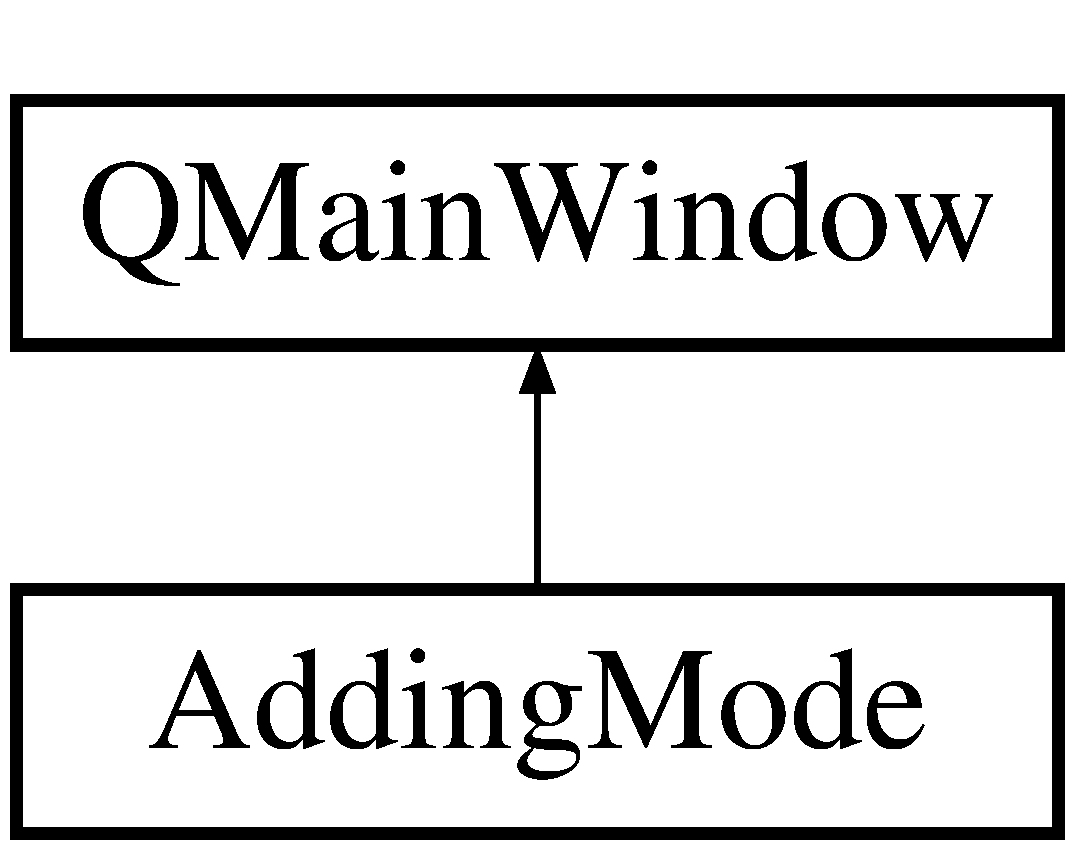
\includegraphics[height=2.000000cm]{class_adding_mode}
\end{center}
\end{figure}
\subsection*{Signals}
\begin{DoxyCompactItemize}
\item 
\mbox{\Hypertarget{class_adding_mode_ac9a9d671ccfc803f9844cde060a12ca5}\label{class_adding_mode_ac9a9d671ccfc803f9844cde060a12ca5}} 
void {\bfseries show\+Event\+Planner} ()
\end{DoxyCompactItemize}
\subsection*{Public Member Functions}
\begin{DoxyCompactItemize}
\item 
\mbox{\Hypertarget{class_adding_mode_aa8830870d671f8d806bedd0ecf03d065}\label{class_adding_mode_aa8830870d671f8d806bedd0ecf03d065}} 
{\bfseries Adding\+Mode} (\hyperlink{class_session}{Session} $\ast$session, Q\+Widget $\ast$parent=0)
\end{DoxyCompactItemize}


The documentation for this class was generated from the following files\+:\begin{DoxyCompactItemize}
\item 
addingmode.\+h\item 
addingmode.\+cpp\end{DoxyCompactItemize}

\hypertarget{class_event}{}\section{Event Class Reference}
\label{class_event}\index{Event@{Event}}


The \hyperlink{class_event}{Event} class.  




{\ttfamily \#include $<$event.\+h$>$}

\subsection*{Public Member Functions}
\begin{DoxyCompactItemize}
\item 
\hyperlink{class_event_a5a40dd4708297f7031e29b39e039ae10}{Event} ()
\begin{DoxyCompactList}\small\item\em \hyperlink{class_event}{Event}. \end{DoxyCompactList}\item 
\hyperlink{class_event_a28e7aab4f7a4f7bd375a63be18b5c44c}{Event} (Q\+String owner, Q\+String event\+Name, int month, int day, int year, Q\+List$<$ \hyperlink{class_time_slot}{Time\+Slot} $>$ time\+Slots)
\begin{DoxyCompactList}\small\item\em \hyperlink{class_event}{Event}. \end{DoxyCompactList}\item 
int \hyperlink{class_event_a29caad464e4a7cf6aa29973ed9345f6d}{get\+Month} () const
\begin{DoxyCompactList}\small\item\em get\+Month \end{DoxyCompactList}\item 
void \hyperlink{class_event_acd9e57cf462362474a5734874c5267e4}{set\+Month} (int month)
\begin{DoxyCompactList}\small\item\em set\+Month \end{DoxyCompactList}\item 
int \hyperlink{class_event_a710a15a86ca734cbd84e77e8d2ed216c}{get\+Day} () const
\begin{DoxyCompactList}\small\item\em get\+Day \end{DoxyCompactList}\item 
void \hyperlink{class_event_a94940b483087e30b440ff2579b285d9c}{set\+Day} (int day)
\begin{DoxyCompactList}\small\item\em set\+Day \end{DoxyCompactList}\item 
int \hyperlink{class_event_a7ddd7775953aeeb58d311d52139c2844}{get\+Year} () const
\begin{DoxyCompactList}\small\item\em get\+Year \end{DoxyCompactList}\item 
void \hyperlink{class_event_adf16c1b8925ab210055ba0e3c05576d6}{set\+Year} (int year)
\begin{DoxyCompactList}\small\item\em set\+Year \end{DoxyCompactList}\item 
Q\+String \hyperlink{class_event_ab7e1dc08bd691aaf95ad994afdea6d2b}{get\+Owner} () const
\begin{DoxyCompactList}\small\item\em get\+Owner \end{DoxyCompactList}\item 
void \hyperlink{class_event_a4c5b75b1d4c162cb7489ee6a4ced8af0}{set\+Owner} (Q\+String owner)
\begin{DoxyCompactList}\small\item\em set\+Owner \end{DoxyCompactList}\item 
Q\+String \hyperlink{class_event_a2846f2dfad84c083d829fdf3d915c05a}{get\+Event\+Name} ()
\begin{DoxyCompactList}\small\item\em get\+Event\+Name \end{DoxyCompactList}\item 
void \hyperlink{class_event_a15b675acab68dd6a840421ec72aeef57}{set\+Event\+Name} (Q\+String event\+Name)
\begin{DoxyCompactList}\small\item\em set\+Event\+Name \end{DoxyCompactList}\item 
Q\+List$<$ \hyperlink{class_time_slot}{Time\+Slot} $>$ \hyperlink{class_event_a1d54b94176660fa89f06e47de4f38f91}{get\+Time\+Slots} ()
\begin{DoxyCompactList}\small\item\em get\+Time\+Slots \end{DoxyCompactList}\item 
void \hyperlink{class_event_a4e0b462c919ef361c1bce8aa6f806b77}{set\+Time\+Slots} (Q\+List$<$ \hyperlink{class_time_slot}{Time\+Slot} $>$ time\+Slots)
\begin{DoxyCompactList}\small\item\em set\+Time\+Slots \end{DoxyCompactList}\end{DoxyCompactItemize}


\subsection{Detailed Description}
The \hyperlink{class_event}{Event} class. 

Class used to store details of an event. 

\subsection{Constructor \& Destructor Documentation}
\mbox{\Hypertarget{class_event_a5a40dd4708297f7031e29b39e039ae10}\label{class_event_a5a40dd4708297f7031e29b39e039ae10}} 
\index{Event@{Event}!Event@{Event}}
\index{Event@{Event}!Event@{Event}}
\subsubsection{\texorpdfstring{Event()}{Event()}\hspace{0.1cm}{\footnotesize\ttfamily [1/2]}}
{\footnotesize\ttfamily Event\+::\+Event (\begin{DoxyParamCaption}{ }\end{DoxyParamCaption})}



\hyperlink{class_event}{Event}. 

Default constructor. Only default initilizations are made. \mbox{\Hypertarget{class_event_a28e7aab4f7a4f7bd375a63be18b5c44c}\label{class_event_a28e7aab4f7a4f7bd375a63be18b5c44c}} 
\index{Event@{Event}!Event@{Event}}
\index{Event@{Event}!Event@{Event}}
\subsubsection{\texorpdfstring{Event()}{Event()}\hspace{0.1cm}{\footnotesize\ttfamily [2/2]}}
{\footnotesize\ttfamily Event\+::\+Event (\begin{DoxyParamCaption}\item[{Q\+String}]{owner,  }\item[{Q\+String}]{event\+Name,  }\item[{int}]{month,  }\item[{int}]{day,  }\item[{int}]{year,  }\item[{Q\+List$<$ \hyperlink{class_time_slot}{Time\+Slot} $>$}]{time\+Slots }\end{DoxyParamCaption})}



\hyperlink{class_event}{Event}. 

Consturctor used to create fully initiallized \hyperlink{class_event}{Event} object. 
\begin{DoxyParams}{Parameters}
{\em owner} & \\
\hline
{\em event\+Name} & \\
\hline
{\em month} & \\
\hline
{\em day} & \\
\hline
{\em year} & \\
\hline
{\em time\+Slots} & \\
\hline
\end{DoxyParams}


\subsection{Member Function Documentation}
\mbox{\Hypertarget{class_event_a710a15a86ca734cbd84e77e8d2ed216c}\label{class_event_a710a15a86ca734cbd84e77e8d2ed216c}} 
\index{Event@{Event}!get\+Day@{get\+Day}}
\index{get\+Day@{get\+Day}!Event@{Event}}
\subsubsection{\texorpdfstring{get\+Day()}{getDay()}}
{\footnotesize\ttfamily int Event\+::get\+Day (\begin{DoxyParamCaption}{ }\end{DoxyParamCaption}) const}



get\+Day 

Returns the day of the month that the event will occur. \begin{DoxyReturn}{Returns}
Integer 
\end{DoxyReturn}
\mbox{\Hypertarget{class_event_a2846f2dfad84c083d829fdf3d915c05a}\label{class_event_a2846f2dfad84c083d829fdf3d915c05a}} 
\index{Event@{Event}!get\+Event\+Name@{get\+Event\+Name}}
\index{get\+Event\+Name@{get\+Event\+Name}!Event@{Event}}
\subsubsection{\texorpdfstring{get\+Event\+Name()}{getEventName()}}
{\footnotesize\ttfamily Q\+String Event\+::get\+Event\+Name (\begin{DoxyParamCaption}{ }\end{DoxyParamCaption})}



get\+Event\+Name 

Returns the name of the event. \begin{DoxyReturn}{Returns}
Q\+String 
\end{DoxyReturn}
\mbox{\Hypertarget{class_event_a29caad464e4a7cf6aa29973ed9345f6d}\label{class_event_a29caad464e4a7cf6aa29973ed9345f6d}} 
\index{Event@{Event}!get\+Month@{get\+Month}}
\index{get\+Month@{get\+Month}!Event@{Event}}
\subsubsection{\texorpdfstring{get\+Month()}{getMonth()}}
{\footnotesize\ttfamily int Event\+::get\+Month (\begin{DoxyParamCaption}{ }\end{DoxyParamCaption}) const}



get\+Month 

Returns the month that the event will occur. \begin{DoxyReturn}{Returns}
Integer 
\end{DoxyReturn}
\mbox{\Hypertarget{class_event_ab7e1dc08bd691aaf95ad994afdea6d2b}\label{class_event_ab7e1dc08bd691aaf95ad994afdea6d2b}} 
\index{Event@{Event}!get\+Owner@{get\+Owner}}
\index{get\+Owner@{get\+Owner}!Event@{Event}}
\subsubsection{\texorpdfstring{get\+Owner()}{getOwner()}}
{\footnotesize\ttfamily Q\+String Event\+::get\+Owner (\begin{DoxyParamCaption}{ }\end{DoxyParamCaption}) const}



get\+Owner 

Returns the name of the person who created the event. \begin{DoxyReturn}{Returns}
Q\+String 
\end{DoxyReturn}
\mbox{\Hypertarget{class_event_a1d54b94176660fa89f06e47de4f38f91}\label{class_event_a1d54b94176660fa89f06e47de4f38f91}} 
\index{Event@{Event}!get\+Time\+Slots@{get\+Time\+Slots}}
\index{get\+Time\+Slots@{get\+Time\+Slots}!Event@{Event}}
\subsubsection{\texorpdfstring{get\+Time\+Slots()}{getTimeSlots()}}
{\footnotesize\ttfamily Q\+List$<$ \hyperlink{class_time_slot}{Time\+Slot} $>$ Event\+::get\+Time\+Slots (\begin{DoxyParamCaption}{ }\end{DoxyParamCaption})}



get\+Time\+Slots 

Returns the private member Q\+List$<$\+Time\+Slot$>$ time\+Slots. \begin{DoxyReturn}{Returns}
Q\+List$<$\+Time\+Slot$>$ 
\end{DoxyReturn}
\mbox{\Hypertarget{class_event_a7ddd7775953aeeb58d311d52139c2844}\label{class_event_a7ddd7775953aeeb58d311d52139c2844}} 
\index{Event@{Event}!get\+Year@{get\+Year}}
\index{get\+Year@{get\+Year}!Event@{Event}}
\subsubsection{\texorpdfstring{get\+Year()}{getYear()}}
{\footnotesize\ttfamily int Event\+::get\+Year (\begin{DoxyParamCaption}{ }\end{DoxyParamCaption}) const}



get\+Year 

Returns the year that the event will occur. \begin{DoxyReturn}{Returns}
Integer 
\end{DoxyReturn}
\mbox{\Hypertarget{class_event_a94940b483087e30b440ff2579b285d9c}\label{class_event_a94940b483087e30b440ff2579b285d9c}} 
\index{Event@{Event}!set\+Day@{set\+Day}}
\index{set\+Day@{set\+Day}!Event@{Event}}
\subsubsection{\texorpdfstring{set\+Day()}{setDay()}}
{\footnotesize\ttfamily void Event\+::set\+Day (\begin{DoxyParamCaption}\item[{int}]{day }\end{DoxyParamCaption})}



set\+Day 


\begin{DoxyParams}{Parameters}
{\em day} & \\
\hline
\end{DoxyParams}
Sets private variable day to the passed integer. \mbox{\Hypertarget{class_event_a15b675acab68dd6a840421ec72aeef57}\label{class_event_a15b675acab68dd6a840421ec72aeef57}} 
\index{Event@{Event}!set\+Event\+Name@{set\+Event\+Name}}
\index{set\+Event\+Name@{set\+Event\+Name}!Event@{Event}}
\subsubsection{\texorpdfstring{set\+Event\+Name()}{setEventName()}}
{\footnotesize\ttfamily void Event\+::set\+Event\+Name (\begin{DoxyParamCaption}\item[{Q\+String}]{event\+Name }\end{DoxyParamCaption})}



set\+Event\+Name 

Sets private variable event\+Name to the passed Q\+String. 
\begin{DoxyParams}{Parameters}
{\em event\+Name} & \\
\hline
\end{DoxyParams}
\mbox{\Hypertarget{class_event_acd9e57cf462362474a5734874c5267e4}\label{class_event_acd9e57cf462362474a5734874c5267e4}} 
\index{Event@{Event}!set\+Month@{set\+Month}}
\index{set\+Month@{set\+Month}!Event@{Event}}
\subsubsection{\texorpdfstring{set\+Month()}{setMonth()}}
{\footnotesize\ttfamily void Event\+::set\+Month (\begin{DoxyParamCaption}\item[{int}]{month }\end{DoxyParamCaption})}



set\+Month 


\begin{DoxyParams}{Parameters}
{\em month} & \\
\hline
\end{DoxyParams}
Sets private variable month to the passed integer. \mbox{\Hypertarget{class_event_a4c5b75b1d4c162cb7489ee6a4ced8af0}\label{class_event_a4c5b75b1d4c162cb7489ee6a4ced8af0}} 
\index{Event@{Event}!set\+Owner@{set\+Owner}}
\index{set\+Owner@{set\+Owner}!Event@{Event}}
\subsubsection{\texorpdfstring{set\+Owner()}{setOwner()}}
{\footnotesize\ttfamily void Event\+::set\+Owner (\begin{DoxyParamCaption}\item[{Q\+String}]{owner }\end{DoxyParamCaption})}



set\+Owner 

Sets private variable owner to the passed Q\+String. 
\begin{DoxyParams}{Parameters}
{\em owner} & \\
\hline
\end{DoxyParams}
\mbox{\Hypertarget{class_event_a4e0b462c919ef361c1bce8aa6f806b77}\label{class_event_a4e0b462c919ef361c1bce8aa6f806b77}} 
\index{Event@{Event}!set\+Time\+Slots@{set\+Time\+Slots}}
\index{set\+Time\+Slots@{set\+Time\+Slots}!Event@{Event}}
\subsubsection{\texorpdfstring{set\+Time\+Slots()}{setTimeSlots()}}
{\footnotesize\ttfamily void Event\+::set\+Time\+Slots (\begin{DoxyParamCaption}\item[{Q\+List$<$ \hyperlink{class_time_slot}{Time\+Slot} $>$}]{time\+Slots }\end{DoxyParamCaption})}



set\+Time\+Slots 

Sets private variable time\+Slots to the passed Q\+List$<$\+Time\+Slot$>$. 
\begin{DoxyParams}{Parameters}
{\em time\+Slots} & \\
\hline
\end{DoxyParams}
\mbox{\Hypertarget{class_event_adf16c1b8925ab210055ba0e3c05576d6}\label{class_event_adf16c1b8925ab210055ba0e3c05576d6}} 
\index{Event@{Event}!set\+Year@{set\+Year}}
\index{set\+Year@{set\+Year}!Event@{Event}}
\subsubsection{\texorpdfstring{set\+Year()}{setYear()}}
{\footnotesize\ttfamily void Event\+::set\+Year (\begin{DoxyParamCaption}\item[{int}]{year }\end{DoxyParamCaption})}



set\+Year 


\begin{DoxyParams}{Parameters}
{\em year} & \\
\hline
\end{DoxyParams}
Sets private variable year to the passed integer. 

The documentation for this class was generated from the following files\+:\begin{DoxyCompactItemize}
\item 
event.\+h\item 
event.\+cpp\end{DoxyCompactItemize}

\hypertarget{class_event_admin_mode}{}\section{Event\+Admin\+Mode Class Reference}
\label{class_event_admin_mode}\index{Event\+Admin\+Mode@{Event\+Admin\+Mode}}


The \hyperlink{class_event_admin_mode}{Event\+Admin\+Mode} class  Q\+Main\+Window.  




{\ttfamily \#include $<$eventadminmode.\+h$>$}

Inheritance diagram for Event\+Admin\+Mode\+:\begin{figure}[H]
\begin{center}
\leavevmode
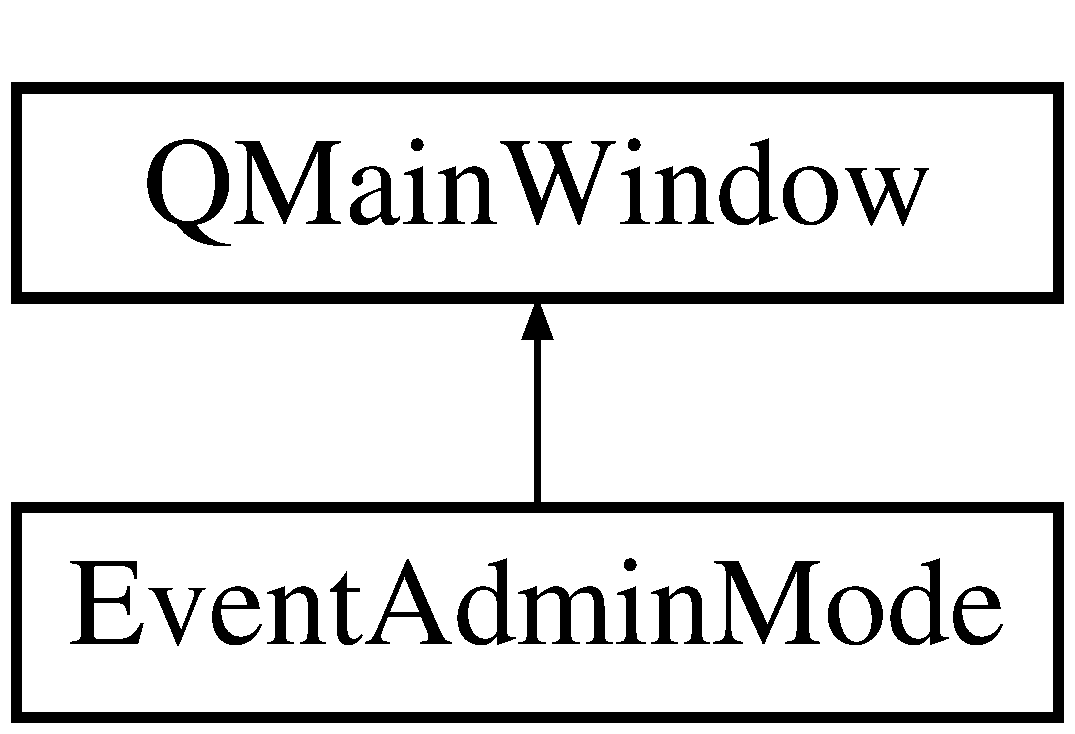
\includegraphics[height=2.000000cm]{class_event_admin_mode}
\end{center}
\end{figure}
\subsection*{Signals}
\begin{DoxyCompactItemize}
\item 
void \hyperlink{class_event_admin_mode_aff26ca6ac01a61846ccef0e55cc274de}{show\+Event\+Planner} ()
\begin{DoxyCompactList}\small\item\em show\+Event\+Planner \end{DoxyCompactList}\item 
void \hyperlink{class_event_admin_mode_a5fcf257db5008a3f634c3fcd13f06994}{quit} ()
\begin{DoxyCompactList}\small\item\em quit \end{DoxyCompactList}\end{DoxyCompactItemize}
\subsection*{Public Member Functions}
\begin{DoxyCompactItemize}
\item 
\hyperlink{class_event_admin_mode_a6f7d4e143b04287d436e9be16324626d}{Event\+Admin\+Mode} (\hyperlink{class_session}{Session} $\ast$session, Q\+Widget $\ast$parent=0)
\begin{DoxyCompactList}\small\item\em \hyperlink{class_event_admin_mode}{Event\+Admin\+Mode}. \end{DoxyCompactList}\item 
Q\+String \hyperlink{class_event_admin_mode_ac659c776c70f4b7f8d6c05ba29b1ae7d}{Info\+\_\+\+Collect} (Q\+String \&Event\+Name, Q\+String \&person\+\_\+name, int month, int day, int year)
\begin{DoxyCompactList}\small\item\em Info\+\_\+\+Collect. \end{DoxyCompactList}\item 
void \hyperlink{class_event_admin_mode_a8e7abbf82a05352cacc29d544a682139}{set\+Style\+\_\+calendar\+Widget} ()
\begin{DoxyCompactList}\small\item\em set\+Style\+\_\+calendar\+Widget \end{DoxyCompactList}\end{DoxyCompactItemize}


\subsection{Detailed Description}
The \hyperlink{class_event_admin_mode}{Event\+Admin\+Mode} class  Q\+Main\+Window. 

Window used for creating new events. 

\subsection{Constructor \& Destructor Documentation}
\mbox{\Hypertarget{class_event_admin_mode_a6f7d4e143b04287d436e9be16324626d}\label{class_event_admin_mode_a6f7d4e143b04287d436e9be16324626d}} 
\index{Event\+Admin\+Mode@{Event\+Admin\+Mode}!Event\+Admin\+Mode@{Event\+Admin\+Mode}}
\index{Event\+Admin\+Mode@{Event\+Admin\+Mode}!Event\+Admin\+Mode@{Event\+Admin\+Mode}}
\subsubsection{\texorpdfstring{Event\+Admin\+Mode()}{EventAdminMode()}}
{\footnotesize\ttfamily Event\+Admin\+Mode\+::\+Event\+Admin\+Mode (\begin{DoxyParamCaption}\item[{\hyperlink{class_session}{Session} $\ast$}]{session,  }\item[{Q\+Widget $\ast$}]{parent = {\ttfamily 0} }\end{DoxyParamCaption})\hspace{0.3cm}{\ttfamily [explicit]}}



\hyperlink{class_event_admin_mode}{Event\+Admin\+Mode}. 

Constructor for \hyperlink{class_event_admin_mode}{Event\+Admin\+Mode} 
\begin{DoxyParams}{Parameters}
{\em session} & \\
\hline
{\em parent} & \\
\hline
\end{DoxyParams}


\subsection{Member Function Documentation}
\mbox{\Hypertarget{class_event_admin_mode_ac659c776c70f4b7f8d6c05ba29b1ae7d}\label{class_event_admin_mode_ac659c776c70f4b7f8d6c05ba29b1ae7d}} 
\index{Event\+Admin\+Mode@{Event\+Admin\+Mode}!Info\+\_\+\+Collect@{Info\+\_\+\+Collect}}
\index{Info\+\_\+\+Collect@{Info\+\_\+\+Collect}!Event\+Admin\+Mode@{Event\+Admin\+Mode}}
\subsubsection{\texorpdfstring{Info\+\_\+\+Collect()}{Info\_Collect()}}
{\footnotesize\ttfamily Q\+String Event\+Admin\+Mode\+::\+Info\+\_\+\+Collect (\begin{DoxyParamCaption}\item[{Q\+String \&}]{Event\+Name,  }\item[{Q\+String \&}]{person\+\_\+name,  }\item[{int}]{month,  }\item[{int}]{day,  }\item[{int}]{year }\end{DoxyParamCaption})}



Info\+\_\+\+Collect. 

Formats a Q\+String for displaying \hyperlink{class_event}{Event} contents. 
\begin{DoxyParams}{Parameters}
{\em Event\+Name} & \\
\hline
{\em person\+\_\+name} & \\
\hline
{\em month} & \\
\hline
{\em day} & \\
\hline
{\em year} & \\
\hline
\end{DoxyParams}
\begin{DoxyReturn}{Returns}
Q\+String 
\end{DoxyReturn}
\mbox{\Hypertarget{class_event_admin_mode_a5fcf257db5008a3f634c3fcd13f06994}\label{class_event_admin_mode_a5fcf257db5008a3f634c3fcd13f06994}} 
\index{Event\+Admin\+Mode@{Event\+Admin\+Mode}!quit@{quit}}
\index{quit@{quit}!Event\+Admin\+Mode@{Event\+Admin\+Mode}}
\subsubsection{\texorpdfstring{quit}{quit}}
{\footnotesize\ttfamily void Event\+Admin\+Mode\+::quit (\begin{DoxyParamCaption}{ }\end{DoxyParamCaption})\hspace{0.3cm}{\ttfamily [signal]}}



quit 

Signal to quit \hyperlink{class_event_admin_mode}{Event\+Admin\+Mode}. \mbox{\Hypertarget{class_event_admin_mode_a8e7abbf82a05352cacc29d544a682139}\label{class_event_admin_mode_a8e7abbf82a05352cacc29d544a682139}} 
\index{Event\+Admin\+Mode@{Event\+Admin\+Mode}!set\+Style\+\_\+calendar\+Widget@{set\+Style\+\_\+calendar\+Widget}}
\index{set\+Style\+\_\+calendar\+Widget@{set\+Style\+\_\+calendar\+Widget}!Event\+Admin\+Mode@{Event\+Admin\+Mode}}
\subsubsection{\texorpdfstring{set\+Style\+\_\+calendar\+Widget()}{setStyle\_calendarWidget()}}
{\footnotesize\ttfamily void Event\+Admin\+Mode\+::set\+Style\+\_\+calendar\+Widget (\begin{DoxyParamCaption}{ }\end{DoxyParamCaption})}



set\+Style\+\_\+calendar\+Widget 

Set a style sheet for calender widget. \mbox{\Hypertarget{class_event_admin_mode_aff26ca6ac01a61846ccef0e55cc274de}\label{class_event_admin_mode_aff26ca6ac01a61846ccef0e55cc274de}} 
\index{Event\+Admin\+Mode@{Event\+Admin\+Mode}!show\+Event\+Planner@{show\+Event\+Planner}}
\index{show\+Event\+Planner@{show\+Event\+Planner}!Event\+Admin\+Mode@{Event\+Admin\+Mode}}
\subsubsection{\texorpdfstring{show\+Event\+Planner}{showEventPlanner}}
{\footnotesize\ttfamily void Event\+Admin\+Mode\+::show\+Event\+Planner (\begin{DoxyParamCaption}{ }\end{DoxyParamCaption})\hspace{0.3cm}{\ttfamily [signal]}}



show\+Event\+Planner 

Signal to go back to the \hyperlink{class_event_planner}{Event\+Planner}. 

The documentation for this class was generated from the following files\+:\begin{DoxyCompactItemize}
\item 
eventadminmode.\+h\item 
eventadminmode.\+cpp\end{DoxyCompactItemize}

\hypertarget{class_event_planner}{}\section{Event\+Planner Class Reference}
\label{class_event_planner}\index{Event\+Planner@{Event\+Planner}}


The \hyperlink{class_event_planner}{Event\+Planner} class  Q\+Main\+Window.  




{\ttfamily \#include $<$eventplanner.\+h$>$}

Inheritance diagram for Event\+Planner\+:\begin{figure}[H]
\begin{center}
\leavevmode
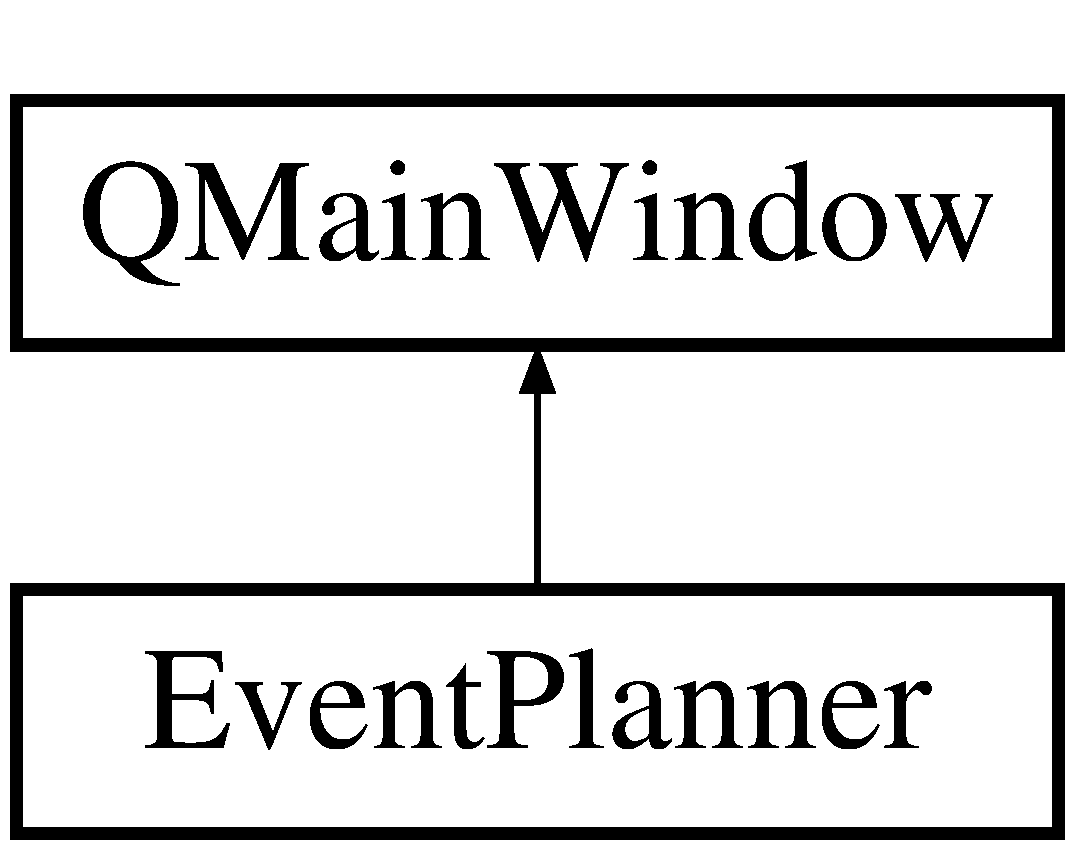
\includegraphics[height=2.000000cm]{class_event_planner}
\end{center}
\end{figure}
\subsection*{Signals}
\begin{DoxyCompactItemize}
\item 
void \hyperlink{class_event_planner_ac29d7162ba23478a3ca83d9a3451317e}{Adding\+Modeshow} ()
\begin{DoxyCompactList}\small\item\em Adding\+Modeshow. \end{DoxyCompactList}\item 
void \hyperlink{class_event_planner_a11d013b57831e685d134d824db883ad3}{Addingn\+Modequit} ()
\begin{DoxyCompactList}\small\item\em Addingn\+Modequit. \end{DoxyCompactList}\item 
void \hyperlink{class_event_planner_ae781e84143069d552b60b7856e7b0ad6}{Admin\+Modeshow} ()
\begin{DoxyCompactList}\small\item\em Admin\+Modeshow. \end{DoxyCompactList}\item 
void \hyperlink{class_event_planner_ab721a944eda1470ebb158bc815cc8734}{Admin\+Modequit} ()
\begin{DoxyCompactList}\small\item\em Admin\+Modequit. \end{DoxyCompactList}\end{DoxyCompactItemize}
\subsection*{Public Member Functions}
\begin{DoxyCompactItemize}
\item 
\hyperlink{class_event_planner_ae8b0e5c382c777476a003e3c099d5e38}{Event\+Planner} (Q\+Widget $\ast$parent=0)
\begin{DoxyCompactList}\small\item\em \hyperlink{class_event_planner}{Event\+Planner}. \end{DoxyCompactList}\item 
\mbox{\Hypertarget{class_event_planner_a2453c0478a2c0f60575e553dbea57f1e}\label{class_event_planner_a2453c0478a2c0f60575e553dbea57f1e}} 
void \hyperlink{class_event_planner_a2453c0478a2c0f60575e553dbea57f1e}{set\+Picture} ()
\begin{DoxyCompactList}\small\item\em set\+Picture  picture to menu screen. \end{DoxyCompactList}\end{DoxyCompactItemize}


\subsection{Detailed Description}
The \hyperlink{class_event_planner}{Event\+Planner} class  Q\+Main\+Window. 

Main menu window with options to either go to \hyperlink{class_event_admin_mode}{Event\+Admin\+Mode} or \hyperlink{class_adding_mode}{Adding\+Mode} 

\subsection{Constructor \& Destructor Documentation}
\mbox{\Hypertarget{class_event_planner_ae8b0e5c382c777476a003e3c099d5e38}\label{class_event_planner_ae8b0e5c382c777476a003e3c099d5e38}} 
\index{Event\+Planner@{Event\+Planner}!Event\+Planner@{Event\+Planner}}
\index{Event\+Planner@{Event\+Planner}!Event\+Planner@{Event\+Planner}}
\subsubsection{\texorpdfstring{Event\+Planner()}{EventPlanner()}}
{\footnotesize\ttfamily Event\+Planner\+::\+Event\+Planner (\begin{DoxyParamCaption}\item[{Q\+Widget $\ast$}]{parent = {\ttfamily 0} }\end{DoxyParamCaption})\hspace{0.3cm}{\ttfamily [explicit]}}



\hyperlink{class_event_planner}{Event\+Planner}. 

Construtor for menu window of main page. 
\begin{DoxyParams}{Parameters}
{\em parent} & \\
\hline
\end{DoxyParams}


\subsection{Member Function Documentation}
\mbox{\Hypertarget{class_event_planner_ac29d7162ba23478a3ca83d9a3451317e}\label{class_event_planner_ac29d7162ba23478a3ca83d9a3451317e}} 
\index{Event\+Planner@{Event\+Planner}!Adding\+Modeshow@{Adding\+Modeshow}}
\index{Adding\+Modeshow@{Adding\+Modeshow}!Event\+Planner@{Event\+Planner}}
\subsubsection{\texorpdfstring{Adding\+Modeshow}{AddingModeshow}}
{\footnotesize\ttfamily void Event\+Planner\+::\+Adding\+Modeshow (\begin{DoxyParamCaption}{ }\end{DoxyParamCaption})\hspace{0.3cm}{\ttfamily [signal]}}



Adding\+Modeshow. 

Signal to switch to Adding Mode for adding availablity \mbox{\Hypertarget{class_event_planner_a11d013b57831e685d134d824db883ad3}\label{class_event_planner_a11d013b57831e685d134d824db883ad3}} 
\index{Event\+Planner@{Event\+Planner}!Addingn\+Modequit@{Addingn\+Modequit}}
\index{Addingn\+Modequit@{Addingn\+Modequit}!Event\+Planner@{Event\+Planner}}
\subsubsection{\texorpdfstring{Addingn\+Modequit}{AddingnModequit}}
{\footnotesize\ttfamily void Event\+Planner\+::\+Addingn\+Modequit (\begin{DoxyParamCaption}{ }\end{DoxyParamCaption})\hspace{0.3cm}{\ttfamily [signal]}}



Addingn\+Modequit. 

Signal that Addinf Mode was left \mbox{\Hypertarget{class_event_planner_ab721a944eda1470ebb158bc815cc8734}\label{class_event_planner_ab721a944eda1470ebb158bc815cc8734}} 
\index{Event\+Planner@{Event\+Planner}!Admin\+Modequit@{Admin\+Modequit}}
\index{Admin\+Modequit@{Admin\+Modequit}!Event\+Planner@{Event\+Planner}}
\subsubsection{\texorpdfstring{Admin\+Modequit}{AdminModequit}}
{\footnotesize\ttfamily void Event\+Planner\+::\+Admin\+Modequit (\begin{DoxyParamCaption}{ }\end{DoxyParamCaption})\hspace{0.3cm}{\ttfamily [signal]}}



Admin\+Modequit. 

Signal to say that Admin mode was exitted \mbox{\Hypertarget{class_event_planner_ae781e84143069d552b60b7856e7b0ad6}\label{class_event_planner_ae781e84143069d552b60b7856e7b0ad6}} 
\index{Event\+Planner@{Event\+Planner}!Admin\+Modeshow@{Admin\+Modeshow}}
\index{Admin\+Modeshow@{Admin\+Modeshow}!Event\+Planner@{Event\+Planner}}
\subsubsection{\texorpdfstring{Admin\+Modeshow}{AdminModeshow}}
{\footnotesize\ttfamily void Event\+Planner\+::\+Admin\+Modeshow (\begin{DoxyParamCaption}{ }\end{DoxyParamCaption})\hspace{0.3cm}{\ttfamily [signal]}}



Admin\+Modeshow. 

Signal to show Admin mode for creating events 

The documentation for this class was generated from the following files\+:\begin{DoxyCompactItemize}
\item 
eventplanner.\+h\item 
eventplanner.\+cpp\end{DoxyCompactItemize}

\hypertarget{class_session}{}\section{Session Class Reference}
\label{class_session}\index{Session@{Session}}


The \hyperlink{class_session}{Session} class.  




{\ttfamily \#include $<$session.\+h$>$}

\subsection*{Public Member Functions}
\begin{DoxyCompactItemize}
\item 
\hyperlink{class_session_ad92ef09b872c9227e38a6efdd4d8a837}{Session} ()
\begin{DoxyCompactList}\small\item\em \hyperlink{class_session}{Session}. \end{DoxyCompactList}\item 
\hyperlink{class_session_a0a7362dd58b94a67af892eb2cda1082a}{Session} (Q\+String user)
\begin{DoxyCompactList}\small\item\em \hyperlink{class_session}{Session}. \end{DoxyCompactList}\item 
void \hyperlink{class_session_aaeaa643e010cc10517063cd031412ec4}{add\+Event} (Q\+String owner, Q\+String event\+Name, int month, int day, int year, Q\+List$<$ \hyperlink{class_time_slot}{Time\+Slot} $>$ time\+Slots)
\begin{DoxyCompactList}\small\item\em add\+Event \end{DoxyCompactList}\item 
bool \hyperlink{class_session_aff9fd19eb09a0ac22d3e2c2615f9f9e9}{read\+Events\+From\+File} ()
\begin{DoxyCompactList}\small\item\em read\+Events\+From\+File \end{DoxyCompactList}\item 
bool \hyperlink{class_session_af095af8449dd10f6fdf3db6d530e109e}{save\+Events\+To\+File} ()
\begin{DoxyCompactList}\small\item\em save\+Events\+To\+File \end{DoxyCompactList}\item 
Q\+String \hyperlink{class_session_a09e51bffb8d4657efcb8ccf47be3192d}{get\+User} () const
\begin{DoxyCompactList}\small\item\em get\+User \end{DoxyCompactList}\item 
void \hyperlink{class_session_a3e4500bdcf80458ae14dde3eb413adb8}{set\+User} (Q\+String user)
\begin{DoxyCompactList}\small\item\em set\+User \end{DoxyCompactList}\item 
std\+::list$<$ \hyperlink{class_event}{Event} $\ast$ $>$ \& \hyperlink{class_session_a9712e356f0d5c3efdaed996ddc063738}{get\+Events} ()
\begin{DoxyCompactList}\small\item\em get\+Events \end{DoxyCompactList}\item 
int \hyperlink{class_session_aa6766de9b237384f6eff9ccbdfd8bde9}{number\+Of\+Events} () const
\begin{DoxyCompactList}\small\item\em number\+Of\+Events \end{DoxyCompactList}\end{DoxyCompactItemize}


\subsection{Detailed Description}
The \hyperlink{class_session}{Session} class. 

The session object is used to handle reading and writing events to file for storage as well as stroing events in memory while program is running. 

\subsection{Constructor \& Destructor Documentation}
\mbox{\Hypertarget{class_session_ad92ef09b872c9227e38a6efdd4d8a837}\label{class_session_ad92ef09b872c9227e38a6efdd4d8a837}} 
\index{Session@{Session}!Session@{Session}}
\index{Session@{Session}!Session@{Session}}
\subsubsection{\texorpdfstring{Session()}{Session()}\hspace{0.1cm}{\footnotesize\ttfamily [1/2]}}
{\footnotesize\ttfamily Session\+::\+Session (\begin{DoxyParamCaption}{ }\end{DoxyParamCaption})}



\hyperlink{class_session}{Session}. 

Default constructor. All initializations are set to default. \mbox{\Hypertarget{class_session_a0a7362dd58b94a67af892eb2cda1082a}\label{class_session_a0a7362dd58b94a67af892eb2cda1082a}} 
\index{Session@{Session}!Session@{Session}}
\index{Session@{Session}!Session@{Session}}
\subsubsection{\texorpdfstring{Session()}{Session()}\hspace{0.1cm}{\footnotesize\ttfamily [2/2]}}
{\footnotesize\ttfamily Session\+::\+Session (\begin{DoxyParamCaption}\item[{Q\+String}]{user }\end{DoxyParamCaption})}



\hyperlink{class_session}{Session}. 

Constructor where private memebr variable Q\+String user is set to the passed argument. 
\begin{DoxyParams}{Parameters}
{\em user} & \\
\hline
\end{DoxyParams}


\subsection{Member Function Documentation}
\mbox{\Hypertarget{class_session_aaeaa643e010cc10517063cd031412ec4}\label{class_session_aaeaa643e010cc10517063cd031412ec4}} 
\index{Session@{Session}!add\+Event@{add\+Event}}
\index{add\+Event@{add\+Event}!Session@{Session}}
\subsubsection{\texorpdfstring{add\+Event()}{addEvent()}}
{\footnotesize\ttfamily void Session\+::add\+Event (\begin{DoxyParamCaption}\item[{Q\+String}]{owner,  }\item[{Q\+String}]{event\+Name,  }\item[{int}]{month,  }\item[{int}]{day,  }\item[{int}]{year,  }\item[{Q\+List$<$ \hyperlink{class_time_slot}{Time\+Slot} $>$}]{time\+Slots }\end{DoxyParamCaption})}



add\+Event 

Creates a new \hyperlink{class_event}{Event} using the passed arguments and pushes it to the end of private memeber variable td\+::list$<$\+Event$\ast$$>$ events. 
\begin{DoxyParams}{Parameters}
{\em owner} & \\
\hline
{\em event\+Name} & \\
\hline
{\em month} & \\
\hline
{\em day} & \\
\hline
{\em year} & \\
\hline
{\em time\+Slots} & \\
\hline
\end{DoxyParams}
\mbox{\Hypertarget{class_session_a9712e356f0d5c3efdaed996ddc063738}\label{class_session_a9712e356f0d5c3efdaed996ddc063738}} 
\index{Session@{Session}!get\+Events@{get\+Events}}
\index{get\+Events@{get\+Events}!Session@{Session}}
\subsubsection{\texorpdfstring{get\+Events()}{getEvents()}}
{\footnotesize\ttfamily std\+::list$<$ \hyperlink{class_event}{Event} $\ast$ $>$ \& Session\+::get\+Events (\begin{DoxyParamCaption}{ }\end{DoxyParamCaption})}



get\+Events 

Returns the private member variable std\+::list$<$\+Event$\ast$$>$ events. This is a list of \hyperlink{class_event}{Event} pointers of all Events avaivalbe in the \hyperlink{class_session}{Session}. \begin{DoxyReturn}{Returns}
std\+::list$<$\+Event$\ast$$>$ 
\end{DoxyReturn}
\mbox{\Hypertarget{class_session_a09e51bffb8d4657efcb8ccf47be3192d}\label{class_session_a09e51bffb8d4657efcb8ccf47be3192d}} 
\index{Session@{Session}!get\+User@{get\+User}}
\index{get\+User@{get\+User}!Session@{Session}}
\subsubsection{\texorpdfstring{get\+User()}{getUser()}}
{\footnotesize\ttfamily Q\+String Session\+::get\+User (\begin{DoxyParamCaption}{ }\end{DoxyParamCaption}) const}



get\+User 

Returns the private member Q\+String user. \begin{DoxyReturn}{Returns}
Q\+String 
\end{DoxyReturn}
\mbox{\Hypertarget{class_session_aa6766de9b237384f6eff9ccbdfd8bde9}\label{class_session_aa6766de9b237384f6eff9ccbdfd8bde9}} 
\index{Session@{Session}!number\+Of\+Events@{number\+Of\+Events}}
\index{number\+Of\+Events@{number\+Of\+Events}!Session@{Session}}
\subsubsection{\texorpdfstring{number\+Of\+Events()}{numberOfEvents()}}
{\footnotesize\ttfamily int Session\+::number\+Of\+Events (\begin{DoxyParamCaption}{ }\end{DoxyParamCaption}) const}



number\+Of\+Events 

Returns the size of std\+::list$<$\+Event$\ast$$>$ events. \begin{DoxyReturn}{Returns}
int 
\end{DoxyReturn}
\mbox{\Hypertarget{class_session_aff9fd19eb09a0ac22d3e2c2615f9f9e9}\label{class_session_aff9fd19eb09a0ac22d3e2c2615f9f9e9}} 
\index{Session@{Session}!read\+Events\+From\+File@{read\+Events\+From\+File}}
\index{read\+Events\+From\+File@{read\+Events\+From\+File}!Session@{Session}}
\subsubsection{\texorpdfstring{read\+Events\+From\+File()}{readEventsFromFile()}}
{\footnotesize\ttfamily bool Session\+::read\+Events\+From\+File (\begin{DoxyParamCaption}{ }\end{DoxyParamCaption})}



read\+Events\+From\+File 

Reads in contents of Event\+Data.\+txt and parses for \hyperlink{class_event}{Event} objects. Events objects are the pushed into std\+::list$<$\+Event$\ast$$>$ events. \begin{DoxyReturn}{Returns}
True if file succesfully parsed. False otherwise. 
\end{DoxyReturn}
\mbox{\Hypertarget{class_session_af095af8449dd10f6fdf3db6d530e109e}\label{class_session_af095af8449dd10f6fdf3db6d530e109e}} 
\index{Session@{Session}!save\+Events\+To\+File@{save\+Events\+To\+File}}
\index{save\+Events\+To\+File@{save\+Events\+To\+File}!Session@{Session}}
\subsubsection{\texorpdfstring{save\+Events\+To\+File()}{saveEventsToFile()}}
{\footnotesize\ttfamily bool Session\+::save\+Events\+To\+File (\begin{DoxyParamCaption}{ }\end{DoxyParamCaption})}



save\+Events\+To\+File 

Writes formatted contents of std\+::list$<$\+Event$\ast$$>$ events to file Event\+Data.\+txt. \begin{DoxyReturn}{Returns}
True if file succesfully saved. False otherwise. 
\end{DoxyReturn}
\mbox{\Hypertarget{class_session_a3e4500bdcf80458ae14dde3eb413adb8}\label{class_session_a3e4500bdcf80458ae14dde3eb413adb8}} 
\index{Session@{Session}!set\+User@{set\+User}}
\index{set\+User@{set\+User}!Session@{Session}}
\subsubsection{\texorpdfstring{set\+User()}{setUser()}}
{\footnotesize\ttfamily void Session\+::set\+User (\begin{DoxyParamCaption}\item[{Q\+String}]{user }\end{DoxyParamCaption})}



set\+User 

Sets the private member variable Q\+String user to the passed argument. 
\begin{DoxyParams}{Parameters}
{\em user} & \\
\hline
\end{DoxyParams}


The documentation for this class was generated from the following files\+:\begin{DoxyCompactItemize}
\item 
session.\+h\item 
session.\+cpp\end{DoxyCompactItemize}

\hypertarget{class_time_slot}{}\section{Time\+Slot Class Reference}
\label{class_time_slot}\index{Time\+Slot@{Time\+Slot}}


The \hyperlink{class_time_slot}{Time\+Slot} class.  




{\ttfamily \#include $<$timeslot.\+h$>$}

\subsection*{Public Member Functions}
\begin{DoxyCompactItemize}
\item 
\hyperlink{class_time_slot_a8bdfc0039c8da76edc16c4a1070bdc80}{Time\+Slot} ()
\begin{DoxyCompactList}\small\item\em \hyperlink{class_time_slot}{Time\+Slot}. \end{DoxyCompactList}\item 
void \hyperlink{class_time_slot_a7b0ee031f73b9f6eb40fee11939b9a7e}{add\+Attendee} (Q\+String attendee)
\begin{DoxyCompactList}\small\item\em add\+Attendee \end{DoxyCompactList}\item 
Q\+String\+List \hyperlink{class_time_slot_a01c092d21d983b5b67cf2678f54d2c74}{get\+Attendees} () const
\begin{DoxyCompactList}\small\item\em get\+Attendees \end{DoxyCompactList}\item 
Q\+String \hyperlink{class_time_slot_a23c04da070ed921bf66396da1d958547}{get\+Time12\+Hour} () const
\begin{DoxyCompactList}\small\item\em get\+Time12\+Hour \end{DoxyCompactList}\item 
void \hyperlink{class_time_slot_a9b50d81d78b54b9127029e7fffba198b}{set\+Time12\+Hour} (Q\+String time)
\begin{DoxyCompactList}\small\item\em set\+Time12\+Hour \end{DoxyCompactList}\item 
Q\+String \hyperlink{class_time_slot_aec0c82baaf408509d976307fa682e6ce}{get\+Time24\+Hour} () const
\begin{DoxyCompactList}\small\item\em get\+Time24\+Hour \end{DoxyCompactList}\item 
void \hyperlink{class_time_slot_aa095348bd53bd45ca4797181e6927ea4}{set\+Time24\+Hour} (Q\+String time)
\begin{DoxyCompactList}\small\item\em set\+Time24\+Hour \end{DoxyCompactList}\item 
bool \hyperlink{class_time_slot_a7448b6ba71a8b1107dffa98365d593aa}{is\+Selected} () const
\begin{DoxyCompactList}\small\item\em is\+Selected \end{DoxyCompactList}\item 
void \hyperlink{class_time_slot_aa063569ec2bc23d252a6eacab8f183fc}{set\+True} ()
\begin{DoxyCompactList}\small\item\em set\+True \end{DoxyCompactList}\item 
void \hyperlink{class_time_slot_adb02c968ee765b49136f051a9ea43b06}{set\+False} ()
\begin{DoxyCompactList}\small\item\em set\+False \end{DoxyCompactList}\item 
void \hyperlink{class_time_slot_ab955b538853b38792c502f30beea5d9b}{clear\+Time\+Slot} ()
\begin{DoxyCompactList}\small\item\em clear\+Time\+Slot \end{DoxyCompactList}\item 
void \hyperlink{class_time_slot_a6a28b7702ca5df07ddaf5e25d37b1bd1}{set\+Attendees} (Q\+String\+List attendees)
\begin{DoxyCompactList}\small\item\em set\+Attendees \end{DoxyCompactList}\end{DoxyCompactItemize}


\subsection{Detailed Description}
The \hyperlink{class_time_slot}{Time\+Slot} class. 

Class using to hold information for a single time slot of an event. 

\subsection{Constructor \& Destructor Documentation}
\mbox{\Hypertarget{class_time_slot_a8bdfc0039c8da76edc16c4a1070bdc80}\label{class_time_slot_a8bdfc0039c8da76edc16c4a1070bdc80}} 
\index{Time\+Slot@{Time\+Slot}!Time\+Slot@{Time\+Slot}}
\index{Time\+Slot@{Time\+Slot}!Time\+Slot@{Time\+Slot}}
\subsubsection{\texorpdfstring{Time\+Slot()}{TimeSlot()}}
{\footnotesize\ttfamily Time\+Slot\+::\+Time\+Slot (\begin{DoxyParamCaption}{ }\end{DoxyParamCaption})}



\hyperlink{class_time_slot}{Time\+Slot}. 

Default constructor. Privare bool selected is initialized to false. 

\subsection{Member Function Documentation}
\mbox{\Hypertarget{class_time_slot_a7b0ee031f73b9f6eb40fee11939b9a7e}\label{class_time_slot_a7b0ee031f73b9f6eb40fee11939b9a7e}} 
\index{Time\+Slot@{Time\+Slot}!add\+Attendee@{add\+Attendee}}
\index{add\+Attendee@{add\+Attendee}!Time\+Slot@{Time\+Slot}}
\subsubsection{\texorpdfstring{add\+Attendee()}{addAttendee()}}
{\footnotesize\ttfamily void Time\+Slot\+::add\+Attendee (\begin{DoxyParamCaption}\item[{Q\+String}]{attendee }\end{DoxyParamCaption})}



add\+Attendee 

Pushes passed Q\+String onto private membervariable Q\+String\+List attendees. 
\begin{DoxyParams}{Parameters}
{\em attendee} & \\
\hline
\end{DoxyParams}
\mbox{\Hypertarget{class_time_slot_ab955b538853b38792c502f30beea5d9b}\label{class_time_slot_ab955b538853b38792c502f30beea5d9b}} 
\index{Time\+Slot@{Time\+Slot}!clear\+Time\+Slot@{clear\+Time\+Slot}}
\index{clear\+Time\+Slot@{clear\+Time\+Slot}!Time\+Slot@{Time\+Slot}}
\subsubsection{\texorpdfstring{clear\+Time\+Slot()}{clearTimeSlot()}}
{\footnotesize\ttfamily void Time\+Slot\+::clear\+Time\+Slot (\begin{DoxyParamCaption}{ }\end{DoxyParamCaption})}



clear\+Time\+Slot 

Q\+String\+List attendees is cleared of all Q\+Strings and bool selected is set to false. \mbox{\Hypertarget{class_time_slot_a01c092d21d983b5b67cf2678f54d2c74}\label{class_time_slot_a01c092d21d983b5b67cf2678f54d2c74}} 
\index{Time\+Slot@{Time\+Slot}!get\+Attendees@{get\+Attendees}}
\index{get\+Attendees@{get\+Attendees}!Time\+Slot@{Time\+Slot}}
\subsubsection{\texorpdfstring{get\+Attendees()}{getAttendees()}}
{\footnotesize\ttfamily Q\+String\+List Time\+Slot\+::get\+Attendees (\begin{DoxyParamCaption}{ }\end{DoxyParamCaption}) const}



get\+Attendees 

Returns the private membervariable Q\+String\+List attendees. \begin{DoxyReturn}{Returns}
Q\+String\+List 
\end{DoxyReturn}
\mbox{\Hypertarget{class_time_slot_a23c04da070ed921bf66396da1d958547}\label{class_time_slot_a23c04da070ed921bf66396da1d958547}} 
\index{Time\+Slot@{Time\+Slot}!get\+Time12\+Hour@{get\+Time12\+Hour}}
\index{get\+Time12\+Hour@{get\+Time12\+Hour}!Time\+Slot@{Time\+Slot}}
\subsubsection{\texorpdfstring{get\+Time12\+Hour()}{getTime12Hour()}}
{\footnotesize\ttfamily Q\+String Time\+Slot\+::get\+Time12\+Hour (\begin{DoxyParamCaption}{ }\end{DoxyParamCaption}) const}



get\+Time12\+Hour 

Returns the Q\+String that contains the 12 hour clock format of the time slot. \begin{DoxyReturn}{Returns}
Q\+String 
\end{DoxyReturn}
\mbox{\Hypertarget{class_time_slot_aec0c82baaf408509d976307fa682e6ce}\label{class_time_slot_aec0c82baaf408509d976307fa682e6ce}} 
\index{Time\+Slot@{Time\+Slot}!get\+Time24\+Hour@{get\+Time24\+Hour}}
\index{get\+Time24\+Hour@{get\+Time24\+Hour}!Time\+Slot@{Time\+Slot}}
\subsubsection{\texorpdfstring{get\+Time24\+Hour()}{getTime24Hour()}}
{\footnotesize\ttfamily Q\+String Time\+Slot\+::get\+Time24\+Hour (\begin{DoxyParamCaption}{ }\end{DoxyParamCaption}) const}



get\+Time24\+Hour 

Returns the Q\+String that contains the 24 hour clock format of the time slot. \begin{DoxyReturn}{Returns}
Q\+String 
\end{DoxyReturn}
\mbox{\Hypertarget{class_time_slot_a7448b6ba71a8b1107dffa98365d593aa}\label{class_time_slot_a7448b6ba71a8b1107dffa98365d593aa}} 
\index{Time\+Slot@{Time\+Slot}!is\+Selected@{is\+Selected}}
\index{is\+Selected@{is\+Selected}!Time\+Slot@{Time\+Slot}}
\subsubsection{\texorpdfstring{is\+Selected()}{isSelected()}}
{\footnotesize\ttfamily bool Time\+Slot\+::is\+Selected (\begin{DoxyParamCaption}{ }\end{DoxyParamCaption}) const}



is\+Selected 

Returns a bool that represents if the \hyperlink{class_time_slot}{Time\+Slot} has been selected to be part of the \hyperlink{class_event}{Event}. \begin{DoxyReturn}{Returns}
bool 
\end{DoxyReturn}
\mbox{\Hypertarget{class_time_slot_a6a28b7702ca5df07ddaf5e25d37b1bd1}\label{class_time_slot_a6a28b7702ca5df07ddaf5e25d37b1bd1}} 
\index{Time\+Slot@{Time\+Slot}!set\+Attendees@{set\+Attendees}}
\index{set\+Attendees@{set\+Attendees}!Time\+Slot@{Time\+Slot}}
\subsubsection{\texorpdfstring{set\+Attendees()}{setAttendees()}}
{\footnotesize\ttfamily void Time\+Slot\+::set\+Attendees (\begin{DoxyParamCaption}\item[{Q\+String\+List}]{attendees }\end{DoxyParamCaption})}



set\+Attendees 

The private member variable Q\+String\+List attendees is set to the passed argument. 
\begin{DoxyParams}{Parameters}
{\em attendees} & \\
\hline
\end{DoxyParams}
\mbox{\Hypertarget{class_time_slot_adb02c968ee765b49136f051a9ea43b06}\label{class_time_slot_adb02c968ee765b49136f051a9ea43b06}} 
\index{Time\+Slot@{Time\+Slot}!set\+False@{set\+False}}
\index{set\+False@{set\+False}!Time\+Slot@{Time\+Slot}}
\subsubsection{\texorpdfstring{set\+False()}{setFalse()}}
{\footnotesize\ttfamily void Time\+Slot\+::set\+False (\begin{DoxyParamCaption}{ }\end{DoxyParamCaption})}



set\+False 

Set the private member variable bool selected to false. \mbox{\Hypertarget{class_time_slot_a9b50d81d78b54b9127029e7fffba198b}\label{class_time_slot_a9b50d81d78b54b9127029e7fffba198b}} 
\index{Time\+Slot@{Time\+Slot}!set\+Time12\+Hour@{set\+Time12\+Hour}}
\index{set\+Time12\+Hour@{set\+Time12\+Hour}!Time\+Slot@{Time\+Slot}}
\subsubsection{\texorpdfstring{set\+Time12\+Hour()}{setTime12Hour()}}
{\footnotesize\ttfamily void Time\+Slot\+::set\+Time12\+Hour (\begin{DoxyParamCaption}\item[{Q\+String}]{time }\end{DoxyParamCaption})}



set\+Time12\+Hour 

The private memebr variable Q\+String display\+Time12\+Hour is set to the passed Q\+String. 
\begin{DoxyParams}{Parameters}
{\em time} & \\
\hline
\end{DoxyParams}
\mbox{\Hypertarget{class_time_slot_aa095348bd53bd45ca4797181e6927ea4}\label{class_time_slot_aa095348bd53bd45ca4797181e6927ea4}} 
\index{Time\+Slot@{Time\+Slot}!set\+Time24\+Hour@{set\+Time24\+Hour}}
\index{set\+Time24\+Hour@{set\+Time24\+Hour}!Time\+Slot@{Time\+Slot}}
\subsubsection{\texorpdfstring{set\+Time24\+Hour()}{setTime24Hour()}}
{\footnotesize\ttfamily void Time\+Slot\+::set\+Time24\+Hour (\begin{DoxyParamCaption}\item[{Q\+String}]{time }\end{DoxyParamCaption})}



set\+Time24\+Hour 

The private memebr variable Q\+String display\+Time24\+Hour is set to the passed Q\+String. 
\begin{DoxyParams}{Parameters}
{\em time} & \\
\hline
\end{DoxyParams}
\mbox{\Hypertarget{class_time_slot_aa063569ec2bc23d252a6eacab8f183fc}\label{class_time_slot_aa063569ec2bc23d252a6eacab8f183fc}} 
\index{Time\+Slot@{Time\+Slot}!set\+True@{set\+True}}
\index{set\+True@{set\+True}!Time\+Slot@{Time\+Slot}}
\subsubsection{\texorpdfstring{set\+True()}{setTrue()}}
{\footnotesize\ttfamily void Time\+Slot\+::set\+True (\begin{DoxyParamCaption}{ }\end{DoxyParamCaption})}



set\+True 

Set the private member variable bool selected to true. 

The documentation for this class was generated from the following files\+:\begin{DoxyCompactItemize}
\item 
timeslot.\+h\item 
timeslot.\+cpp\end{DoxyCompactItemize}

%--- End generated contents ---

% Index
\backmatter
\newpage
\phantomsection
\clearemptydoublepage
\addcontentsline{toc}{chapter}{Index}
\printindex

\end{document}
